\newtheorem{assumption}{Assumption}
% \newtheorem{theorem}{Theorem}
% \newtheorem{corollary}{Corollary}
% \newtheorem{lemma}{Lemma}
% \newtheorem{definition}{Definition}
% \newtheorem{remark}{Remark}

\appendix

\section{Derivation of Lower Bound}
\label{sec:derivation_of_lower_bound}
\begin{assumption}
The variational distribution $q(\cdot|z)$ satisfies the regularity condition such that, 
for any $\mathbb{P}_{X|z}\in\{\mathbb{P}'_{X|z}\mid \mathbb{E}_{X|z}[|X|^{2}] < \infty\}$,
\begin{align}
    \mathbb{E}_{X|z}\left[\left(\nabla_{x} \log q(x|z)|_{x=X}\right)^{\intercal}\nabla_{x} \log q(x|z)|_{x=X}\right] < \infty,
\end{align}
where $\mathbb{E}_{X|z}$ is a conditional expectation of $X$ given $z$.
\end{assumption}
\begin{remark}
Note that the Gaussian distribution used in our implementation satisfies the regularity condition.
To check the regularity condition of Gaussian distribution, we first compute the gradient as follows,
\begin{align}
    \nabla_{x}& \log q(x|z)|_{x=X}\\
    &= \nabla_{x} \left(C+\frac{1}{2}\log |\Sigma(z)| + \frac{1}{2}(x-\mu(z))^{\intercal}\Sigma(z)^{-1}(x-\mu(z))\right) |_{x=X}\\
    &= \Sigma(z)^{-1}(X-\mu(z)).
\end{align}
Hence, we get,
\begin{align}
    \mathbb{E}_{X|z}&\left[\left(\nabla_{x} \log q(x|z)|_{x=X}\right)^{\intercal}\nabla_{x} \log q(x|z)|_{x=X}\right]\\
    &= \mathbb{E}_{X|z}\left[(X-\mu(z))^{\intercal}\Sigma(z)^{-2}(X-\mu(z))\right] < \infty.
\end{align}
since $\mu(z)$ and $\Sigma(z)$ are finite and $\mathbb{E}_{X|z}[|X|^{2}]$ is bounded.
Hence, the Gaussian distribution satisfies the regularity condition.
\end{remark}

Under the assumption of $q$, we derive the lower bound.
\begin{proof}[Derivation of the Lower Bound]
Based on the regularity condition, we derive the lower bound of the term, $\mathbb{E}_{Z_{f^{*}},Z_{f}}\left[\log q(Z_{f^{*}}\mid Z_{f})\right]$.
Before starting the derivation, let us define $d_{2,\infty}(f,g):=\sup_{x}\|f(x)-g(x)\|_{2}$.
Then, the derivation starts from Taylor's theorem for a differentiable multivariate function.
From Taylor's theorem, there exists a point $c$ such that $c = tx + (1-t)x_{0}$ for some $t\in[0,1]$ and the following equality holds,
\begin{align}
    \log q(x\mid y) = \log q(x_{0}\mid y) + \nabla_{x} \log q(x\mid y)|_{x=c}^{\intercal}(x-x_{0}).
\end{align}
Then, we can derive the following upper bound as follows,
\begin{align}
    \log q(x\mid y) &= \log q(x_{0}\mid y) + \nabla_{x} \log q(x\mid y)|_{x=c}^{\intercal}(x-x_{0})\\
    &\leq \log q(x_{0}\mid y) + \left|\nabla_{x} \log q(x\mid y)|_{x=c}^{\intercal}(x-x_{0})\right|\\
    &\leq \log q(x_{0}\mid y) + \left\|\nabla_{x} \log q(x\mid y)|_{x=c}\right\|_{2}\left\|x-x_{0}\right\|_{2}
\end{align}
By using this bound, we can derive the following lower bound,
\begin{align}
\mathbb{E}_{Z_{f^{*}}, Z_f}&[\log q(Z_{f^{*}}\mid Z_f)]=\mathbb{E}_{X, X'}\left[\log q(f^{*}(X)\mid f(X'))\right]\\
\geq& \mathbb{E}_{X, X'}\left[\log q(f^{0}(X)\mid f(X'))\right] \nonumber\\
&- \mathbb{E}_{X, X'}\left[\left\|\nabla \log q(c(X)\mid f(X'))\right\|_{2}\left\|f^{0}(X)-f^{*}(X)\right\|_{2}\right]\\
\geq& \mathbb{E}_{X, X'}\left[\log q(f^{0}(X)\mid f(X'))\right] \nonumber\\
&- \mathbb{E}_{X, X'}\left[\left\|\nabla \log q(c(X)\mid f(X'))\right\|_{2}\right]d_{2,\infty}(f^{*},f^{0})\\
\geq& \mathbb{E}_{Z_{f^{0}}, Z_f}\left[\log q(Z_{f^{0}}\mid Z_f)\right]- Cd_{2,\infty}(f^{*},f^{0}),
\end{align}
where $c(x)$ is the function between $f^{0}$ and $f^{*}$, which selects the point satisfying Taylor's theorem, and $C$ is a constant derived from the regularity condition.
\end{proof}


\section{Additional Implementation Details}
\label{sec:additional_impl_details}

\subsection{Hyperparameter tuning}

% Since the HP search protocol of DomainBed \cite{gulrajani2020domainbed} requires very heavy computational resources, we adopt the simplified HP search protocol from Cha \etal \cite{cha2021swad}. 

We split the hyperparameters (HPs) into two groups: algorithm-specific HPs and algorithm-agnostic HPs. The algorithm-agnostic HPs consist of batch size, learning rate, dropout, and weight decay, and \method{} has only one algorithm-specific HP, $\lambda$.
To reduce the computational cost, we tune the algorithm-specific HPs and algorithm-agnostic HPs independently. 
We first search algorithm-specific HPs with default algorithm-agnostic HPs, then search algorithm-agnostic HPs with the tuned algorithm-specific HPs.
That is, the $\lambda$ is searched in [1.0, 0.1, 0.01, 0.001] with the batch size of 32, the learning rate of 5e-5, no dropout, and no weight decay. Then, we search algorithm-agnostic HPs with the searched $\lambda$ following Cha \etal \cite{cha2021swad}. They propose reduced HP search space for efficiency compared to DomainBed \cite{gulrajani2020domainbed}. The protocol searches the learning rate in [1e-5, 3e-5, 5e-5], dropout in [0.0, 0.1, 0.5], and weight decay in [1e-4, 1e-6]. The batch size per domain is fixed to 32. Since \method{} is a regularization method, we add a case of no weight decay.

Even though we use the efficient HP search protocol, it still requires heavy computational resources. Therefore, we tune $\lambda$ only for the non-main experiments, including combination with SWAD, combination with various pre-trained backbones, and the case study on \data{Camelyon17}. Also, we use the batch size of 16 for SWAG \cite{singh2022swag} due to the GPU memory limitation. Note that there is room for further performance improvement by intensive HP tuning and additional usage of GPU memory, considering the simplified HP search protocol and limited computational resources.

\subsection{Implementation details}

The variance encoder is initialized to estimate the variance of 0.1. It is chosen by observing the convergence point of the variance.
Softplus function is employed to ensure non-negativity of the variance. Also, we empirically apply the 10 times larger learning rate for the mean and variance encoders than the feature extractor and the classifier.

\subsection{Mutual information estimation}
\label{subsec:mine}

In Section \ref{subsection:mi_with_oracle}, we estimate the mutual information using Mutual Information Neural Estimator (MINE) \cite{belghazi2018mine}. The mutual information is estimated by MINE as follows:

\begin{align}
    \widehat{I(Z_{f^*} ; Z_f})=\sup _{\theta \in \Theta} \mathbb{E}_{\mathbb{P}_{Z_{f^*} Z_f}}\left[T_{\theta}\right]-\log \left(\mathbb{E}_{\mathbb{P}_{Z_{f^*}} \otimes {\mathbb{P}}_{Z_f}}\left[e^{T_{\theta}}\right]\right).
\end{align}

% We collect 

%In this section, we describe the details about the mutual information experiment (Section 2.2). 
For the features $Z_{f^*}$ and $Z_f$, the features after global average pooling are uniformly collected by domains. The statistics network, $T_\theta$, consists of two hidden linear layers with 512 dimensions and ELU activation functions, following \cite{belghazi2018mine}. In the case of fine-tuning, such as ERM$-$, ERM$+$, and \method{}, the models are trained as many as the number of target domains. Therefore, we estimate the mutual information for each model and report their average value.

\section{Additional Analysis and Discussion}

\subsection{Variations on the assumptions of domain generalization}
\begin{table}[h]
\centering
\small
\caption{\small {\bf Performances of class-conditional MIRO.} 
%\data{OH} and \data{TI} indicate \oh{} and \tr{}, respectively.
}
\label{table:cmiro}
\renewcommand{\arraystretch}{1.2}
\setlength{\tabcolsep}{5pt}
\begin{tabular}{l|cccc|c} 
\toprule
\textbf{Algorithm}   & \pacs{}          & \vlcs{}          & \oh{}            & \data{TerraInc}            & \textbf{Avg.}           \\ \midrule
ERM    & 84.2\scriptsize{$\pm0.1$}          & 77.3\scriptsize{$\pm0.1$}          & 67.6\scriptsize{$\pm0.2$}          & 47.8\scriptsize{$\pm0.6$}          & 69.2           \\
MIRO   & \textbf{85.4}\scriptsize{$\pm0.4$}          & \textbf{79.0}\scriptsize{$\pm0.0$} & 70.5\scriptsize{$\pm0.4$}          & \textbf{50.4}\scriptsize{$\pm1.1$} & \textbf{71.3}  \\
C-MIRO & 85.3\scriptsize{$\pm0.5$} & 78.5\scriptsize{$\pm0.5$}          & \textbf{70.8}\scriptsize{$\pm0.3$} & 49.4\scriptsize{$\pm0.3$}          & 71.0 \\
\bottomrule
\end{tabular}
\end{table}

% Considering types of distribution shift is interesting approach. 
% MIRO does not assume any type of distribution shift. 

% 일반적으로, DG 는 source/target label space 가 같다고 가정하고, multiple source domains 가 존재한다고 가정한다.
% 하지만 이외에 다양한 setup variants 가 존재한다.
% 이러한 가정이 깨지는 경우: single-source DG, heterogeneous DG. MIRO 는 pre-trained model 을 활용하는 대신 multiple source domains 에 대한 가정을 하지 않고, classifier 보다 feature extractor 에 집중하는 메소드이기 때문에, DG 의 가정에서 자유롭게 확장 가능하다.
% 추가적인 가정이 들어가는 경우: 구체적인 distribution shift 에 대한 가정이 있는 경우, 이에 맞춰서 우리의 metric 인 MI 를 수정하는게 도움이 될 수 있다. 예를 들어 class-conditional MI.

In general, domain generalization (DG) assumes that there are multiple source domains, source domain labels are available, and the same input has the same label between source and target domains. Here, we can make the variations on the problem settings by changing the assumption. Single-source DG does not assume the multiple source domains \cite{cha2021swad,fan2021adversarially_single_dg}. Several studies try to solve DG problem without domain labels \cite{carlucci2019jigsaw_jigen,cha2021swad,matsuura2020aaai_mixture_mld}. Heterogeneous DG deals with the label set shift, \ie, the same input can have different labels between source and target domains \cite{li2019heteroDG,wang2020interdomain_mixup_icassp_dg}. In this task, it is assumed that a classifier is learnable in the target domain and the methods focus on the feature extractor. The proposed method exploits pre-trained models instead of assuming available multiple source domains or source domain labels, and focuses on the feature extractor instead of the classifier. Therefore, \method{} is directly applicable to single-source DG, DG without domain labels, and heterogeneous DG problems.
On the other hand, we can consider a more specific type of distribution shift. In this case, we may need a different mutual information (MI) strategy. For example, we can employ class-conditional MI for class-conditional distribution shift (C-MIRO) by using $I(Z_{f^*};Z_f|Y)$ instead of $I(Z_{f^*}; Z_f)$.
In Table \ref{table:cmiro}, C-MIRO achieves comparable scores with MIRO and outperforms ERM even though the problem setting is not class-conditional. From the results, we believe that MIRO can be adapted to other distribution shifts by choosing the proper MI strategy.


% In general, domain generalization (DG) only assumes the same input has the same label between source and target domains. 
% %For the concept or model shift ($P_\mathcal{S}(Y|X) \neq P_\mathcal{T}(Y|X)$), we need an additional treatment to handle class set shift for the classifier training. 
% % There are several studies to handle concept or model shift ($P_\mathcal{S}(Y|X) \neq P_\mathcal{T}(Y|X)$), named \textit{heterogeneous DG} \cite{li2019heteroDG}.
% % %In this setup, the label spaces are disjoint between source and target domains. The goal of heterogeneous DG is to learn a robust feature extractor and the classifier is newly trained in the target domain for evaluation. 
% % Since the proposed MI regularization is focused to learn a robust feature extractor, MIRO framework is directly applicable to the heterogeneous DG.
% % This setup was not considered because it is outside the scope of our study, but extending MIRO framework to such setup is interesting future research direction.
% %Therefore, a method with specific assumption may work better in the specific distribution shift.
% % On the other hand, in a situation where a specific distribution shift can be assumed, an additional design suitable for that shift will be helpful.
% However, for different DS, we may need a different MI strategy.
% % However, as \ra suggested, for a specific DS, we may need a different MI strategy.
% % However, an additional design suitable for a specific distribution shift (\ie, $P_\mathcal{S}(Y|X) \neq P_\mathcal{T}(Y|X)$) will be helpful in a situation where the shift can be assumed.
% As an example of other MI, we employ class-conditional MI for class-conditional DS (C-MIRO) by using $I(Z_{f^*};Z_f|Y)$ instead of $I(Z_{f^*}; Z_f)$.
% In the DG setting (not assuming conditional or target shifts), MIRO shows the best score (Table \ref{table:cmiro}). But, C-MIRO also shows the second-best scores and outperforms ERM even though the problem setting is different. From the results, 
% % MIRO may be adaptable to other DS problems with proper MI strategy.
% we may assume that MIRO can be adapted to other DS problems by choosing the proper MI strategy.



\subsection{The relationship between mutual information and domain generalization performance}
\label{subsec:relationship_mi_dg}

\begin{table}
\centering
\centering
\small
\caption{\small {\bf Average accuracies of ERM$-$, ERM$+$, and MIRO in \pacs{}.} ERM$-$ and ERM$+$ indicate ERM without and with pre-trained model, respectively.}
\label{table:mi_acc_corr}
\renewcommand{\arraystretch}{1.1}
\setlength{\tabcolsep}{4pt}
\begin{tabular}{l|ccc} 
\toprule
\textbf{Pre-trained model}             & \textbf{ERM$-$} & \textbf{ERM$+$} & \textbf{MIRO}  \\ \midrule
ResNet-50 \scriptsize{(ImageNet)}         & 51.6 & 84.2 & 85.4  \\
RegNet-16GF \scriptsize{(Instagram-3.6B)} & 51.5 & 89.6 & 97.4  \\
\bottomrule
\end{tabular}
\end{table}

% Conceptually, our objective finds a solution that maximizes the mutual information (MI) with oracle model while maintaining the source domain performance. 
Our method assumes that knowledge of the oracle model helps domain generalization and it is transferable to the target model by maximizing mutual information (MI). These assumptions are quite intuitive, but there is no theoretical guarantee that MI with the oracle model is perfectly aligned with DG performance. Instead, we empirically observe that a high MI model shows better DG performance if the empirical loss constraint of Equation (2) holds; the pre-trained model itself has high MI but does not satisfy this constraint.
Figure \ref{fig:mi} in the main text shows the rankings of MI for ERM$-$, ERM$+$, and MIRO are in order. Table \ref{table:mi_acc_corr} shows that the rankings are the same for accuracies: ERM$-$ (51.6\%), ERM$+$ (84.2\%), and MIRO (85.4\%) in ImageNet pre-trained ResNet and ERM$-$ (51.5\%), ERM$+$ (89.6\%), and MIRO (97.4\%) in Instagram-3.6B pre-trained RegNet, respectively.
% Fig. 1 shows that ranking of MI and acc for ERM$-$, ERM$+$ and MIRO are the same:
% ERM$-$ (51.6\%), ERM$+$ (84.2\%), and MIRO (85.4\%) in IN-PT ResNet, and ERM$-$ (51.5\%), ERM$+$ (89.6\%), and MIRO (97.4\%) in Instagram-PT RegNet.

% \subsection{Sanity check of objective function}

% \begin{figure}
    \centering
    \begin{subfigure}{0.3\linewidth}
        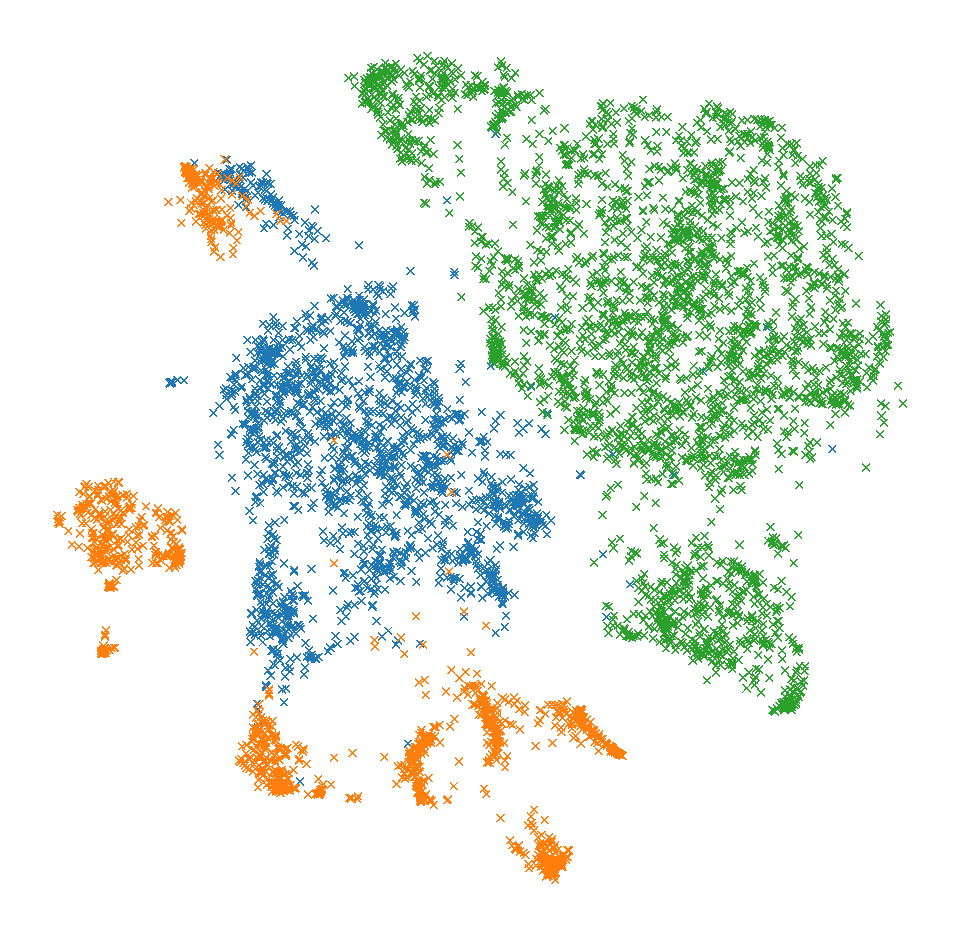
\includegraphics[width=\linewidth]{figures/tsne/PACS_PT.pdf}
        \caption{\small Pre-trained}
        \label{fig:tsne-pretrained}
    \end{subfigure}
    \begin{subfigure}{0.3\linewidth}
        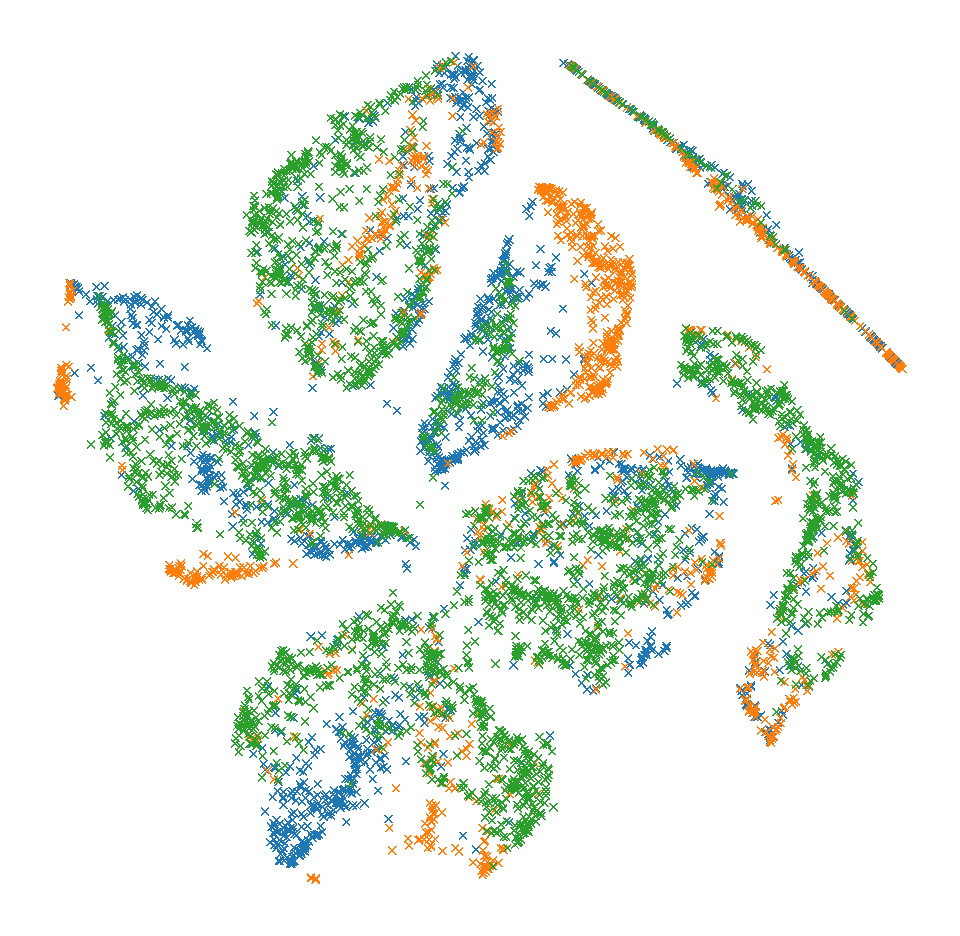
\includegraphics[width=\linewidth]{figures/tsne/PACS_ERM.pdf}
        \caption{\small ERM}
        \label{fig:tsne-erm}
    \end{subfigure}
    % \hfill
    \begin{subfigure}{0.3\linewidth}
        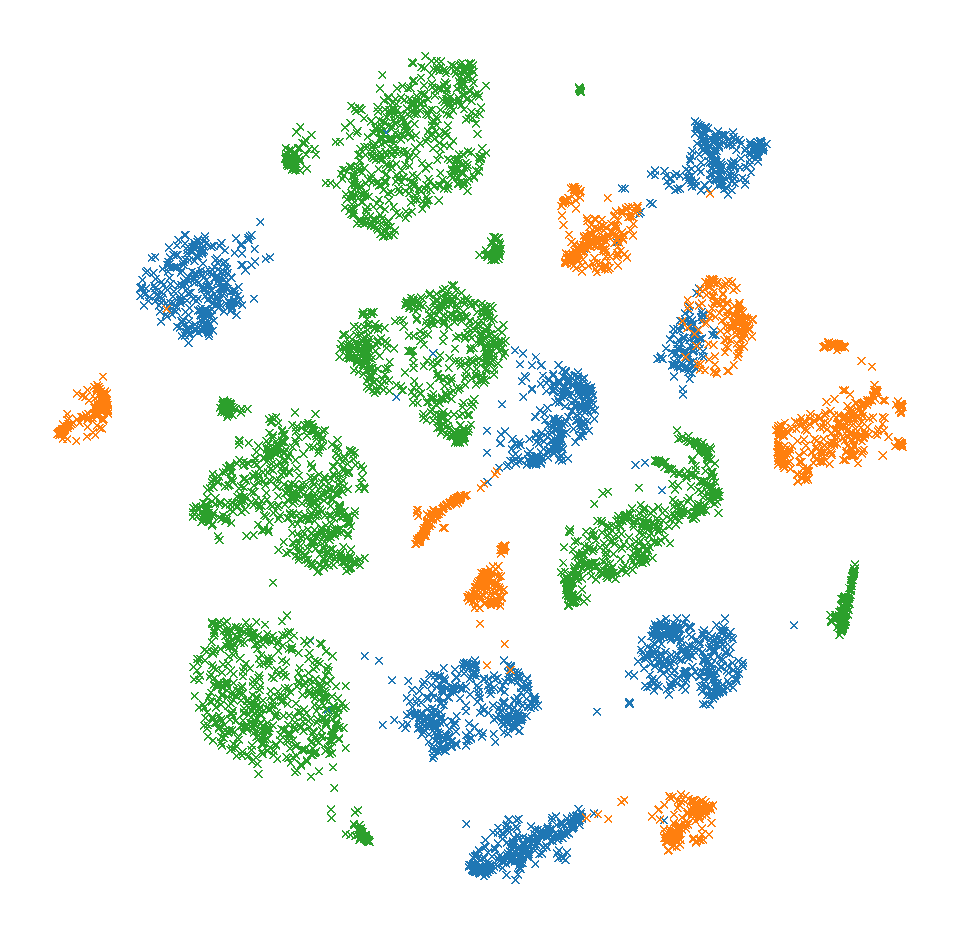
\includegraphics[width=\linewidth]{figures/tsne/PACS_MIRO.pdf}
        \caption{\small MIRO}
        \label{fig:tsne-miro}
    \end{subfigure}
    % \hfill

    \caption{\small \textbf{t-SNE visualization of features in \pacs{}.} Different color indicates different training domain.}
    \label{fig:tsne}
\end{figure}



% \begin{figure}
%     \centering
%     \includegraphics[width=0.7\columnwidth]{figures/mi_all.pdf}
%     \caption{\textbf{Mutual information with oracle model.} \textit{Random} is randomly initialized model, \textit{Scratch} is trained by ERM from \textit{Random}, and \textit{Pretrained} is initialized by pretrained model without training. \textit{ERM} and \textit{SIL} is initialized by pretrained model and trained by each method. $\dagger$ indicates RegNetY-16GF pretrained by SWAG is used and ResNet-50 pretrained in ImageNet is used for the others.}
%     \label{fig:mi}
% \end{figure}





% In this section, we verify our claim that the oracle knowledge is preserved by maximizing mutual information by t-SNE \cite{van2008tsne} visualization.
% Figure \ref{fig:tsne} shows the information preservation effect by MIRO. Features of the pre-trained model are clustered by domain; it means they have domain-specific information. While ERM destroys this information, MIRO preserves it.

% \subsection{Regularization based on mutual information}
% % % MI 는 두 r.v. 의 independence 를 측정하기 위해 널리 사용되었다.
% % % 다른 다양한 대체재가 있지만, MI 는 이론적으로 널리 연구되어 좋은 백그라운드를 제공하며, 동시에 경험적으로도 좋은 결과를 보여왔다 [CITES].
% % % 우리 연구에서도 이러한 맥락에서 MI 를 활용하며, 그 결과 pre-trained model 을 활용한 다른 regularization methods 와 비교했을 때 더 좋은 성능을 내었다.
% % Mutual information is widely used measure to compute dependence between two random variables. 

% Conceptually, our proposed objective Equation (2) can be varying by choosing different metrics rather than MI, such as L1, L2, HSIC, or MMD in feature or parameter spaces \cite{xuhong2018l2sp,li2019delta}.
% We focus on MI because MI theoretically sounds, its approximation works well with a proper theoretical bound, and performs better than others empirically. For example, Table 3 in the main text shows that MI (65.9\%) outperforms weighted L2 in feature space (63.6\%; \cite{li2019delta}) and L2 in parameter space (63.6\%; \cite{xuhong2018l2sp}).
% % Partially yes. We tested several different metrics, such as L1, L2, and weighted L2, in two different spaces, namely feature and weight spaces {\scriptsize [\ct{L2SP}, \ct{DELTA}]}. We found that MI is more principled, better supported theoretically, and shows better results empirically.
% Furthermore, it has been shown in various fields, \eg, domain adaptation and knowledge distillation, that MI is an appropriate metric to transfer information between two representations \cite{ahn2019vid,tian2019crd}. However, there may still exist a metric better than MI. We leave finding the metric better than MI as future work.


\section{Additional Results}

\subsection{Visual comparison between ImageNet and \data{Camelyon17}}
\label{subsec:imagenet_vs_camelyon17}

%% 2-line examples (2x3)
\begin{figure}
\begin{center}
    \begin{subfigure}{0.4\linewidth}
        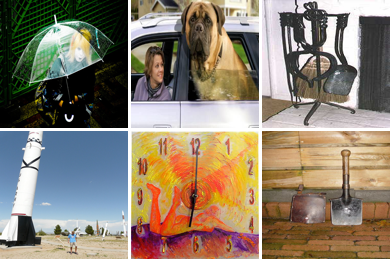
\includegraphics[width=\linewidth]{figures/imagenet_images/2x3grid_IN.png}
        \caption{{ImageNet} (pre-train)}
        \label{fig:imagenet}
    \end{subfigure}
    \quad
    \begin{subfigure}{0.4\linewidth}
        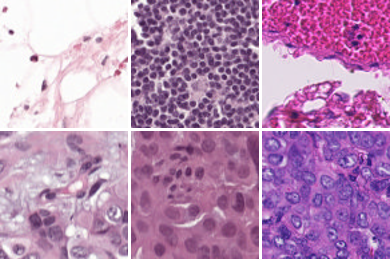
\includegraphics[width=\linewidth]{figures/camelyon_images/2x3grid_CM.png}
        \caption{\data{Camelyon17} (fine-tuning)}
        \label{fig:camelyon}
    \end{subfigure}

    \caption{\small \textbf{Example images of ImageNet and \data{Camelyon17}.} Large distribution shift occurs between pre-training ({ImageNet}) and fine-tuning (\data{Camelyon17}). ImageNet is a multiclass objective recognition task and \data{Camelyon17} is a binary classification task for reading whether the image contains tumor tissue. Instagram-3.6B examples are omitted since it is not publicly available.
    }
    \label{fig:imagenet_camelyon}
\end{center}
\end{figure}


Figure \ref{fig:imagenet_camelyon} shows a huge visual gap between pre-training (ImageNet) and fine-tuning (\data{Camelyon17}) datasets. The tasks are also different; ImageNet is an object recognition task and \data{Camelyon17} is a binary classification of breast cancer. Despite the large gap between pre-training and fine-tuning distribution, the proposed method shows consistent performance improvement (See Table \ref{table:camelyon} in the main text).
%Another pre-training dataset, Instagram-3.6B, is omitted since it is not publicly accessible. 

% This dataset consists of whole-slide images of histological lymph node sections from the five hospitals, where each hospital corresponds to each domain.
% Distribution shifts between hospitals are caused by the way to acquire and process the tissue slide images.
% The task is to predict whether the image contains a tumor tissue of breast cancer. There is a large gap between the pre-training distribution (ImageNet or Instagram-3.6B) and the fine-tuning distribution (\data{Camelyon17}).

\subsection{Relationship between the pre-training scale and the intensity of the mutual information regularization}
\label{subsec:accdiff_by_lambda_more}

In this section, we provide the extended results of Figure \ref{fig:accdiff_varying_lambda} in the main text. Figure \ref{fig:accdiff_varying_lambda_more} shows the additional comparison of three pre-trained backbones according to $\lambda$ about \oh{}, \tr{}, and \dn{}. The comparisons show similar trends with the results in \pacs{}. ImageNet pre-trained backbone, such as ResNet-50 pre-trained in ImageNet \cite{he2016_cvpr_resnet}, has a negative correlation between the performance difference and $\lambda$ in some target domains. Large-scale pre-trained backbones, such as SWAG \cite{singh2022swag} and CLIP \cite{radford2021clip}, tend to consistently make significant performance improvements at high $\lambda$ and become less sensitive to the choice of $\lambda$. 

%Furthermore, it is interesting to note that these trends vary across datasets. In \oh{}, all every backbone has a positive correlation with $\lambda$; if $\lambda$ is increased, the model performance is also increased. In \tr{}, the results are relatively noisy, \eg, SWAG shows the performance degradation at the high $\lambda$. In \dn{}, 

% In the \oh{} dataset, every backbone has a positive correlation with $\lambda$; if $\lambda$ is increased, the model performance is also increased. The results of \tr{} are more noisy than the other datasets. 

\begin{figure}
    \centering
    % \begin{subfigure}{0.9\linewidth}
    %     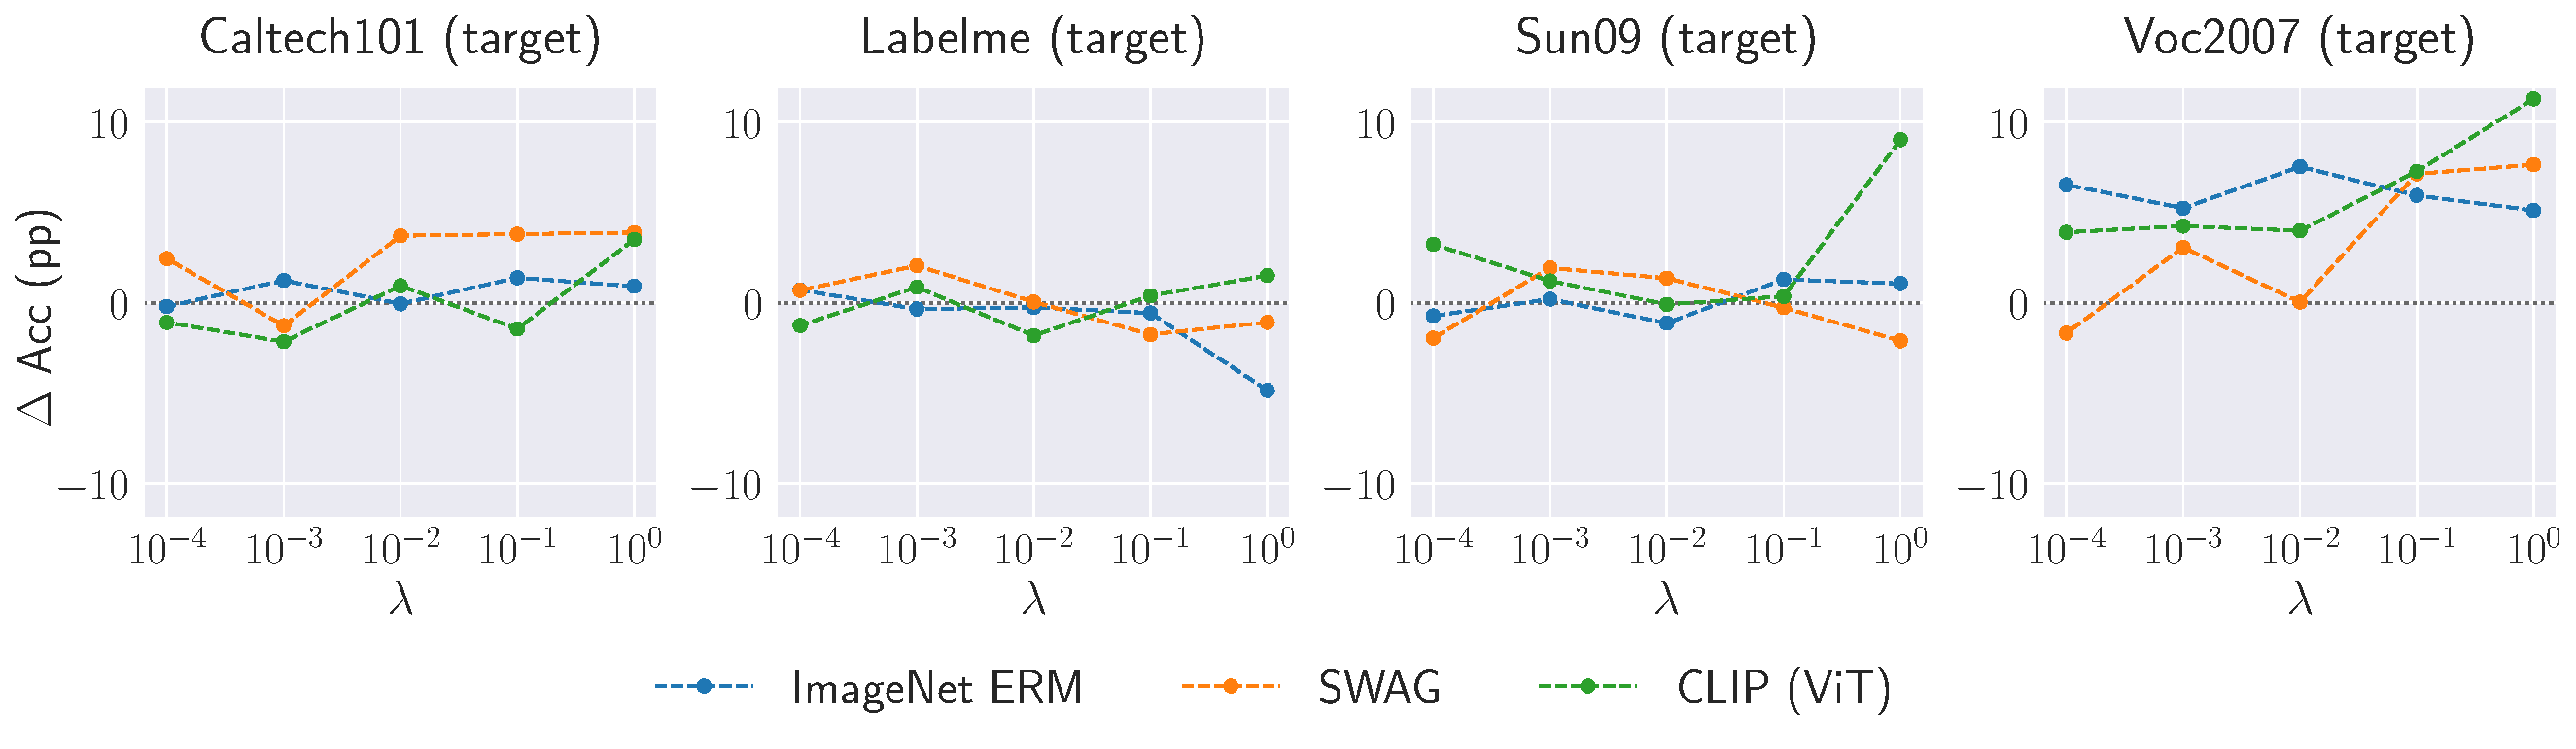
\includegraphics[width=\columnwidth]{figures/accdiff_by_lambda/accdiff_by_lambda_VLCS.pdf}
    %     \caption{\small \vlcs}
    % \end{subfigure}
    \begin{subfigure}{\linewidth}
        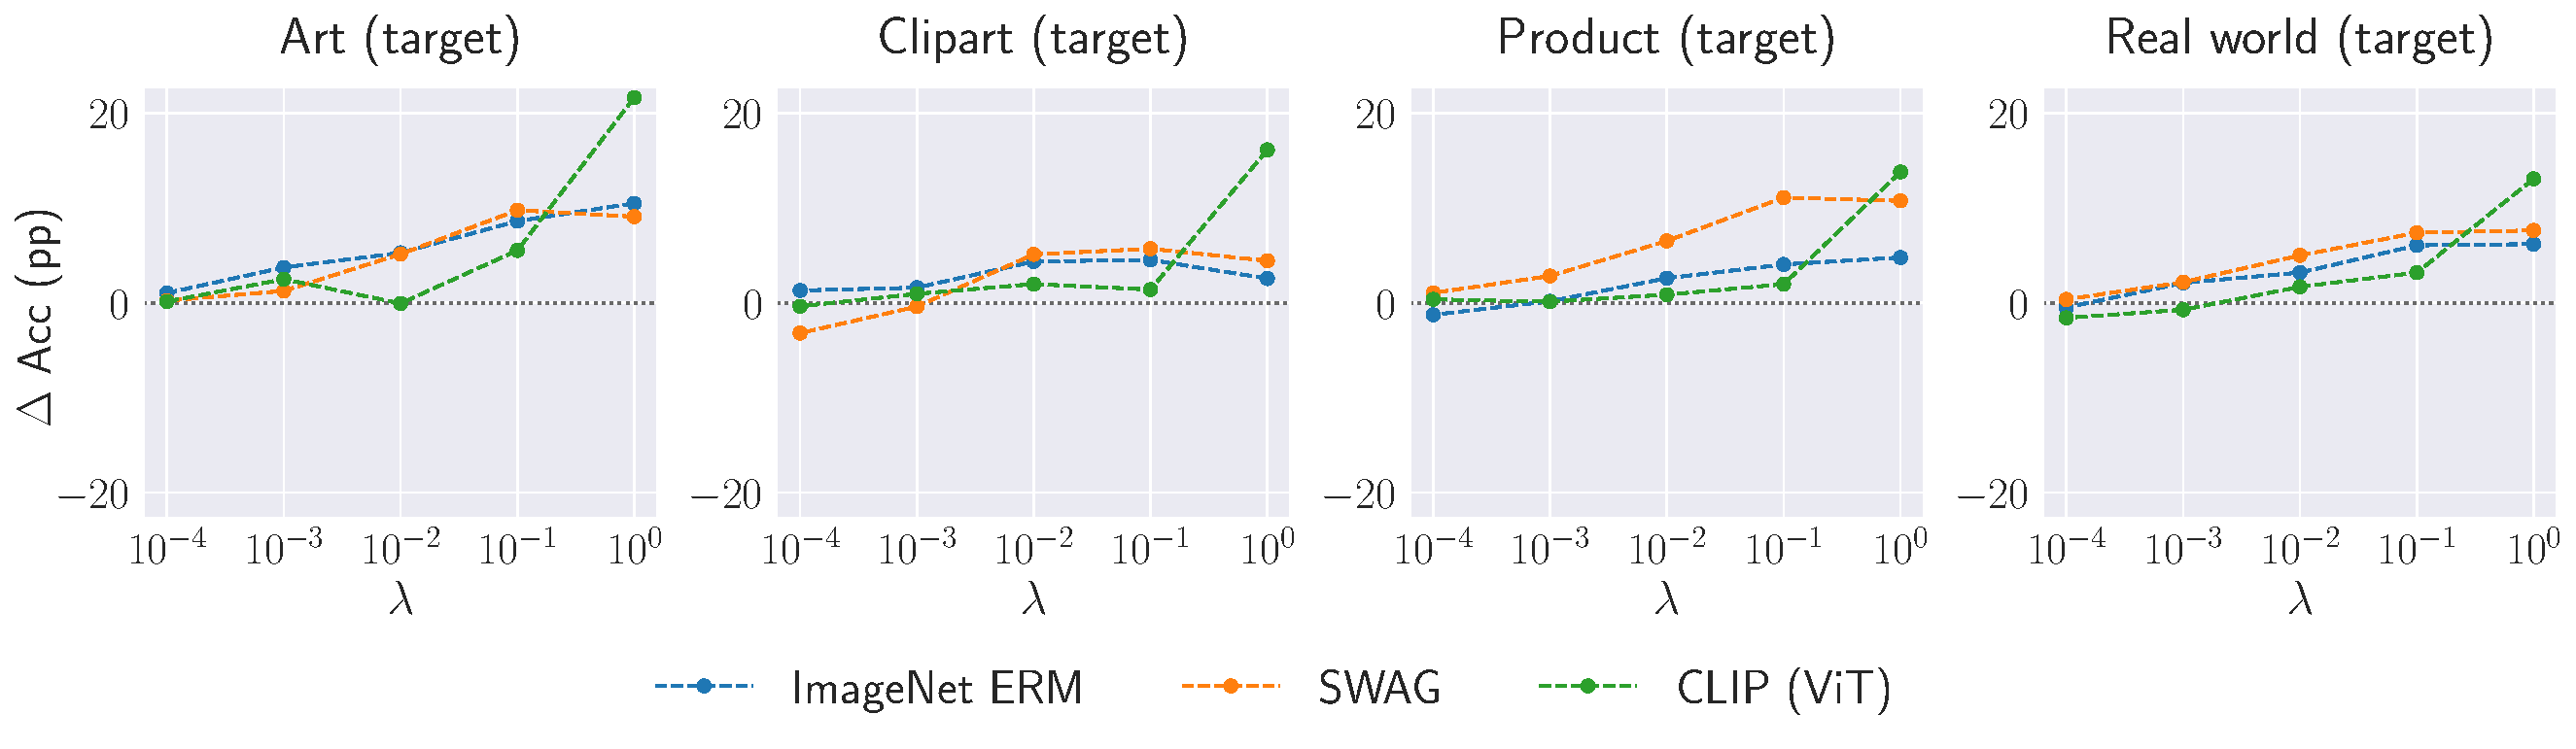
\includegraphics[width=\columnwidth]{figures/accdiff_by_lambda/accdiff_by_lambda_OH.pdf}
        \caption{\small \oh}
    \end{subfigure}
    \begin{subfigure}{\linewidth}
        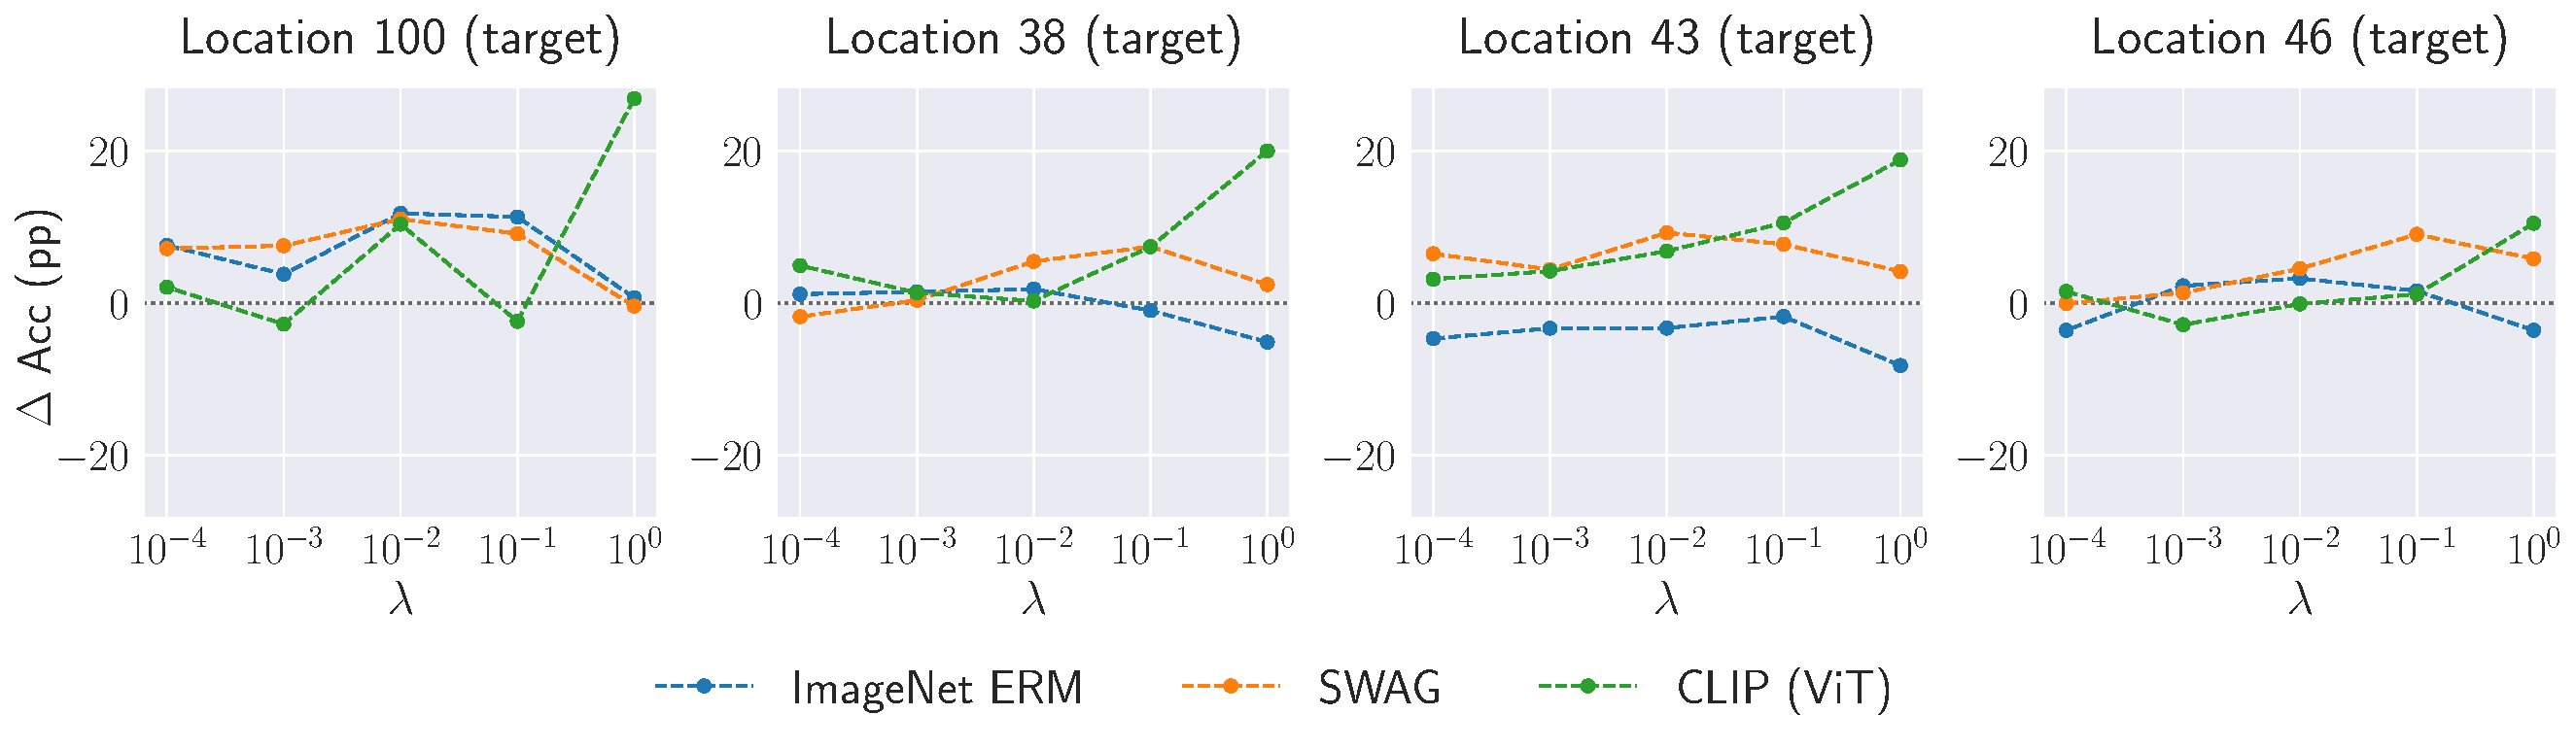
\includegraphics[width=\columnwidth]{figures/accdiff_by_lambda/accdiff_by_lambda_TR.pdf}
        \caption{\small \tr}
    \end{subfigure}
    \begin{subfigure}{0.75\linewidth}
        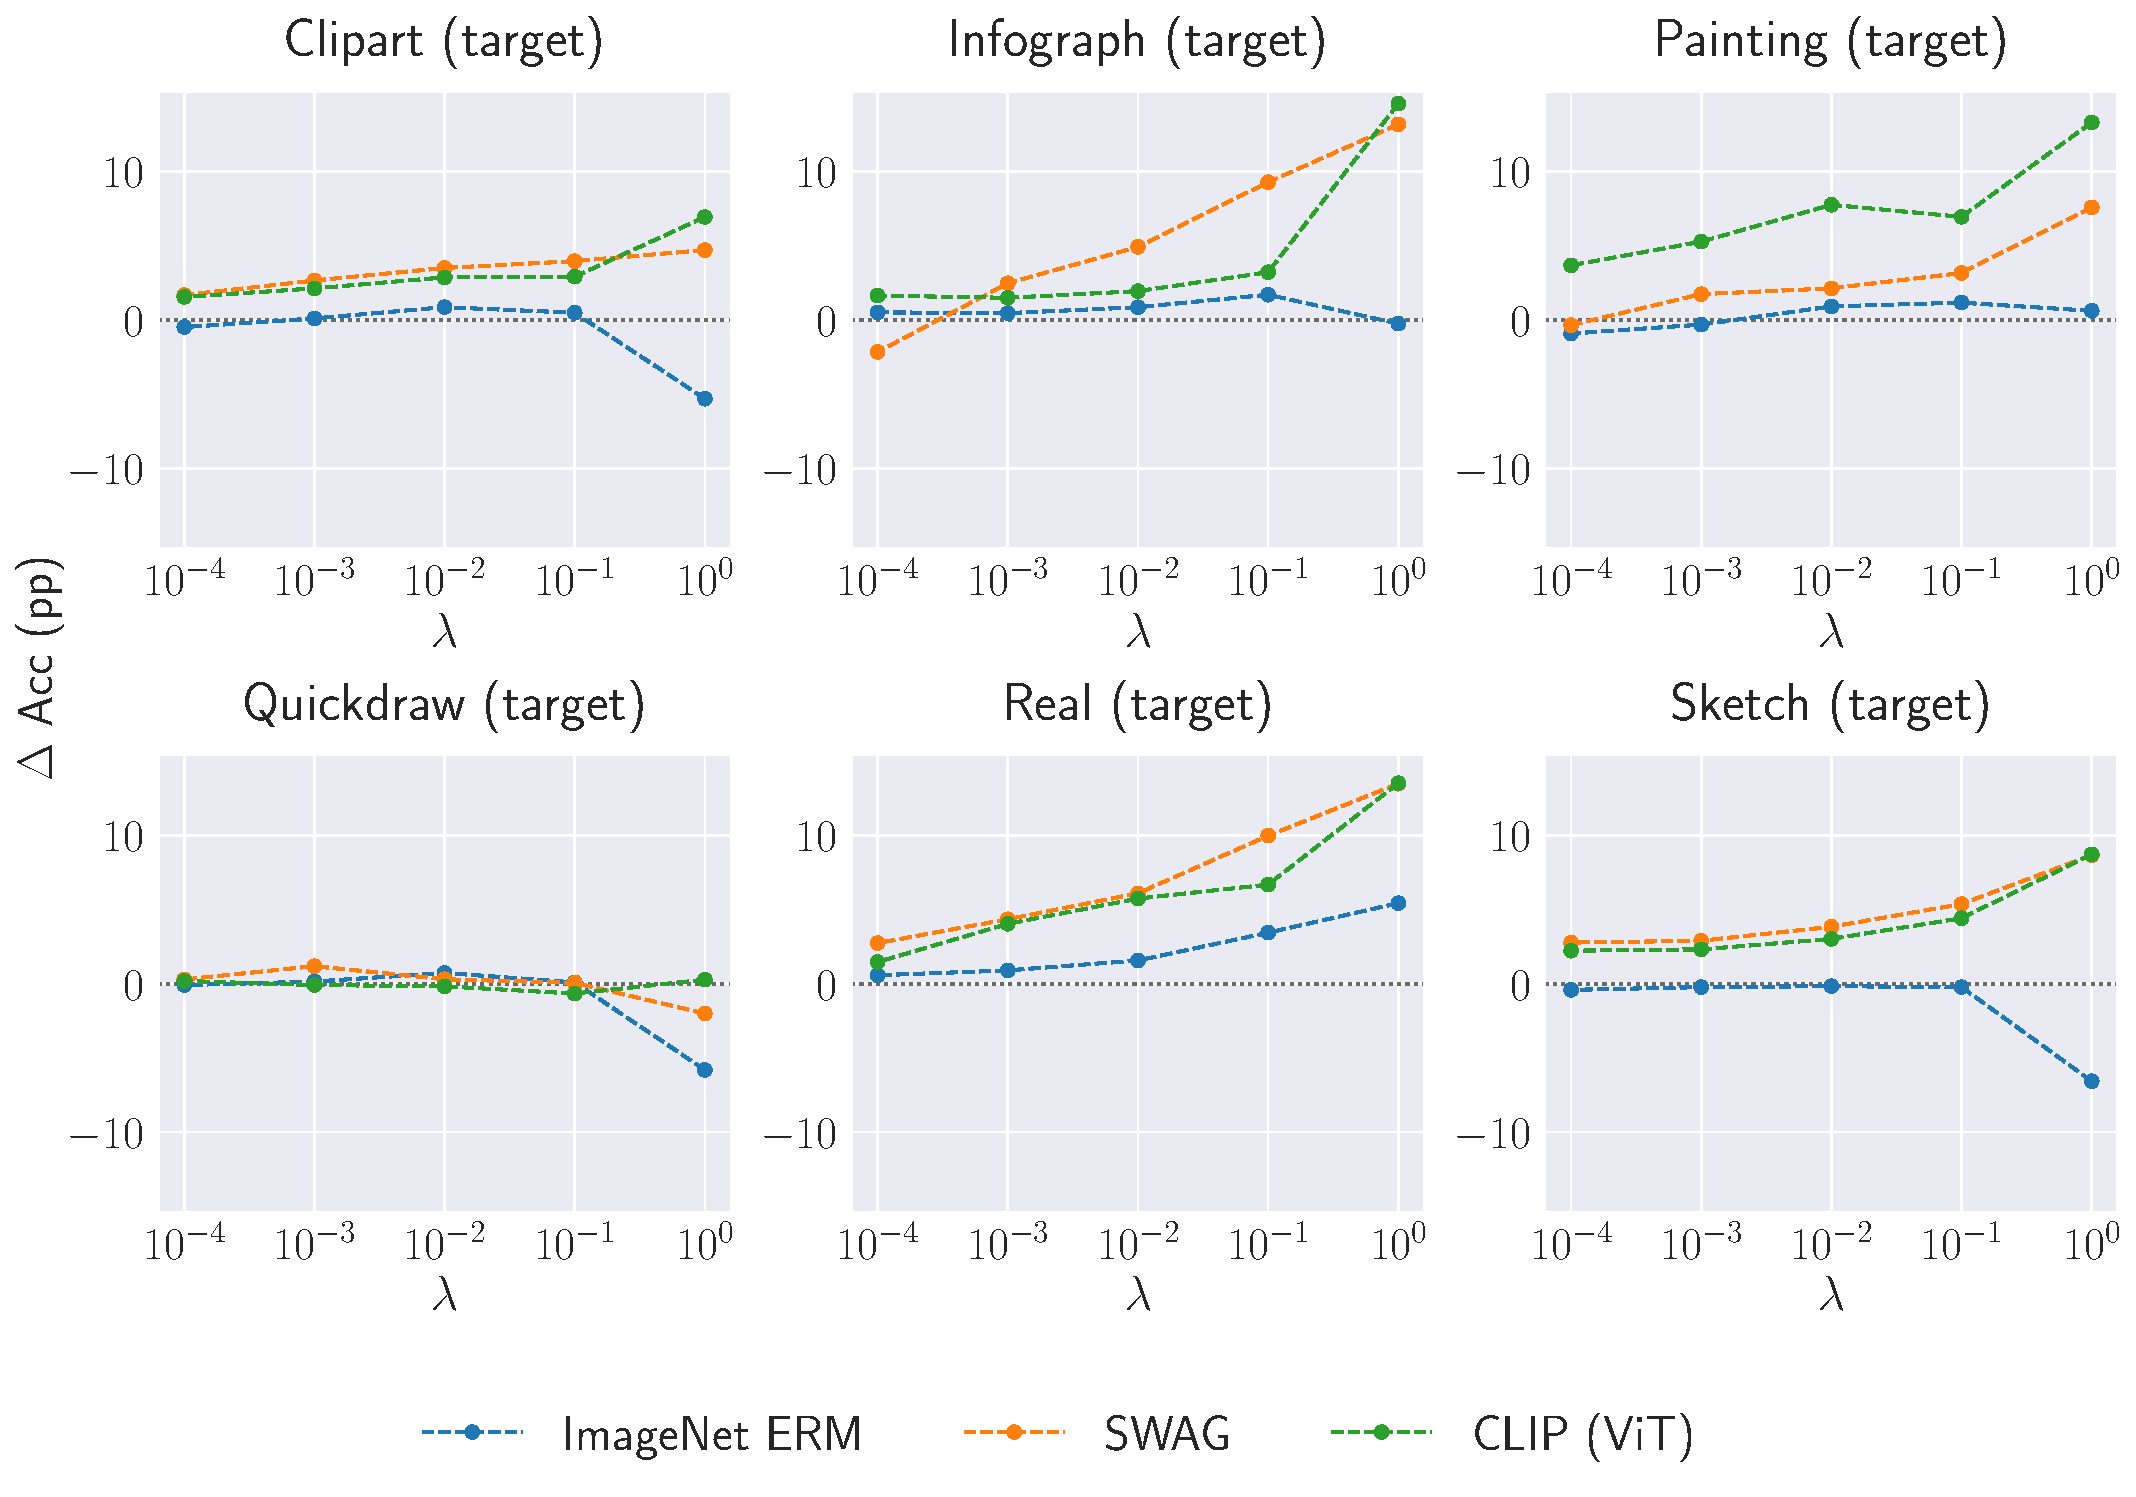
\includegraphics[width=\columnwidth]{figures/accdiff_by_lambda/accdiff_by_lambda_DN.pdf}
        \caption{\small \dn}
    \end{subfigure}

    \caption{\small \textbf{Comparison of three pre-trained models according to $\lambda$.} Y-axis indicates the performance difference of \method{} to ERM. $\lambda$ is the intensity of the mutual information regularization. We compare three models: ResNet-50 pre-trained in ImageNet \cite{he2016_cvpr_resnet}, RegNetY-16GF pre-trained by SWAG \cite{singh2022swag}, and ViT-B pre-trained by CLIP \cite{radford2021clip}.}
    \label{fig:accdiff_varying_lambda_more}
\end{figure}



% \section{Reproducibility}

% For the rigorous reproducibility, we use V100 GPU for the main experiment (Table 1). 

% We provide our source code and detailed environments.
